%%%%%%%%%%%%%%%
% \begin{frame}{}
%   \begin{description}
%     \item[Chapter 6:] Sets
%     \item[Chapter 7:] Operations on Sets
%     \item[Chapter 8:] More on Operations on Sets
%     \item[Chapter 9:] The Power Set and the Cartesian Product
%   \end{description}
% \end{frame}
%%%%%%%%%%%%%%%

%%%%%%%%%%%%%%%
% \begin{frame}{}
%   \begin{center}
%     \resizebox{0.60\textwidth}{!}{\begin{tikzpicture}
\path[mindmap,
    text = white,
    every node/.style = {
      concept,
      circular drop shadow
    },
    root/.style = {
      concept color = red!40,
      font = \Large\bfseries, 
      text width = 8em
    },
    level 1 concept/.append style = {
      concept color = blue!40,
      font = \Large\bfseries,
      sibling angle = 150,
      text width = 8em,
      level distance = 15em,
      inner sep = 0pt
    },
    level 2 concept/.append style = {
      concept color = teal!20,
      font = \bfseries,
      sibling angle = 20,
      level distance = 9em
    },
  ]
  node[root] {Set \\ Theory} [counterclockwise from = 195]
    child[] {
      node {A Branch of Mathematics} [clockwise from = -90]
	% child [] {node (cantor) [] {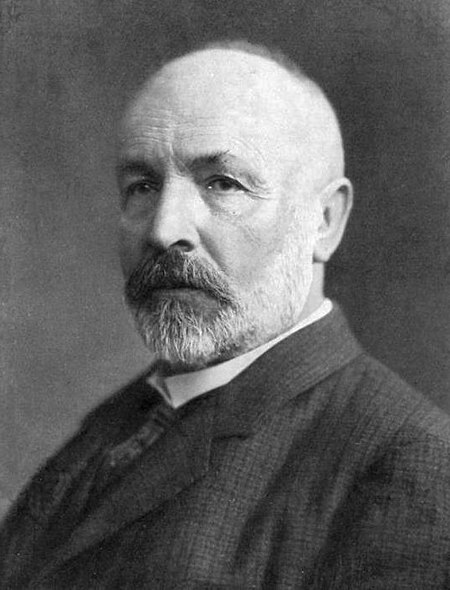
\includegraphics[scale = 0.60]{figs/Cantor}}}
    }
    child[] {
      node {Foundation of Mathematics \\ {\small (+ Logic)}} [counterclockwise from = 195]
	% child [] {node (frege) [] {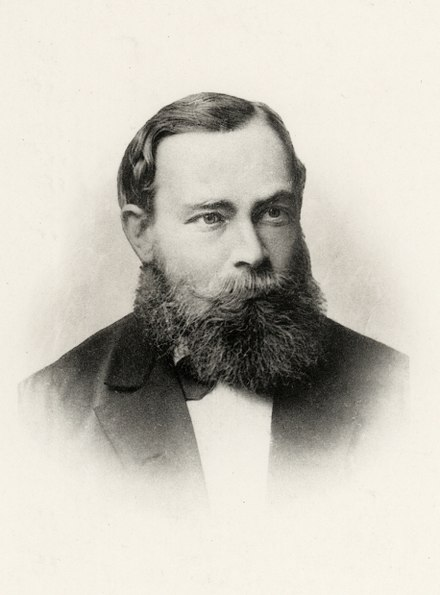
\includegraphics[scale = 0.30]{figs/Frege}}}
	% child [] {node (russell) [] {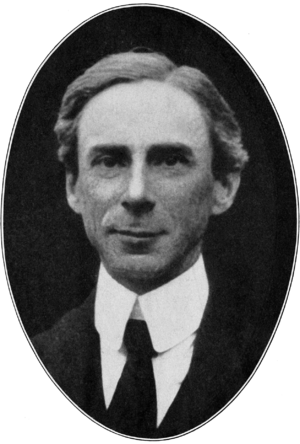
\includegraphics[scale = 0.30]{figs/Russell}}}
	% child [] {node (zermelo) [] {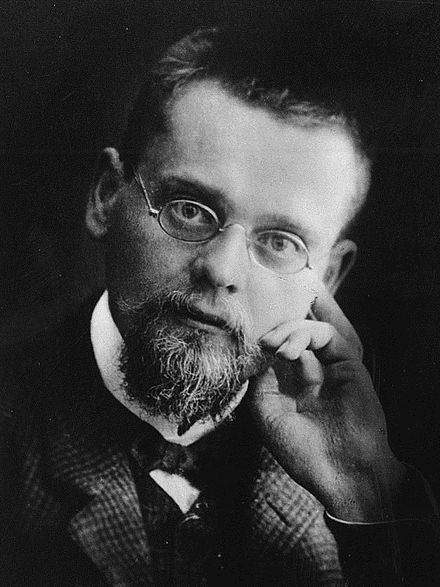
\includegraphics[scale = 0.30]{figs/Zermelo}}}
	% child [] {node (von) [] {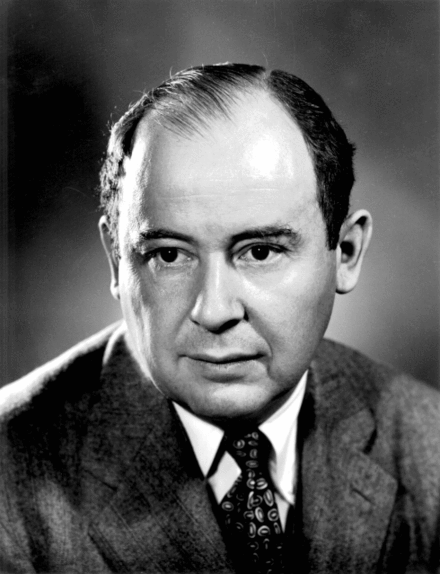
\includegraphics[scale = 0.30]{figs/von-Neumann}}}
    };
\end{tikzpicture}}
%   \end{center}
% 
%   \vspace{-0.50cm}
%   \begin{columns}
%     \pause
%     \column{0.45\textwidth}
%       \fignocaption{width = 0.40\textwidth}{figs/cantor-1870}{\vspace{-0.20cm}\centerline{Georg Cantor}}
%     \pause
%     \column{0.50\textwidth}
%       \begin{columns}
% 	\column{0.50\textwidth}
% 	  \fignocaption{width = 0.50\textwidth}{figs/Frege-old}{\vspace{-0.50cm}\centerline{Gottlob Frege}}
% 	\column{0.50\textwidth}
% 	  \fignocaption{width = 0.50\textwidth}{figs/Russell}{\vspace{-0.50cm}\centerline{Bertrand Russell}}
%       \end{columns}
%       \begin{columns}
% 	\column{0.50\textwidth}
% 	  \fignocaption{width = 0.50\textwidth}{figs/Zermelo-old}{\vspace{-0.50cm}\centerline{Ernst Zermelo}}
% 	\column{0.50\textwidth}
% 	  \fignocaption{width = 0.50\textwidth}{figs/von-Neumann}{\vspace{-0.50cm}\centerline{John von Neumann}}
%       \end{columns}
%   \end{columns}
% \end{frame}
%%%%%%%%%%%%%%%

%%%%%%%%%%%%%%%
\begin{frame}{}
  \begin{columns}
    \column{0.45\textwidth}
      \fignocaption{width = 0.50\textwidth}{figs/Frege-old}{\centerline{Gottlob Frege (1848--1925)}}
    \column{0.45\textwidth}
      \pause
      \fignocaption{width = 0.45\textwidth}{figs/frege-arithmetic}{\centerline{``Basic Laws of Arithmetic''}}
  \end{columns}

  \pause
  \vspace{0.80cm}
  \begin{quote}
    对于一个科学工作者来说,最不幸的事情莫过于:
    当他的工作接近完成时, 却发现那大厦的基础已经动摇。
    \hfill -- 《附录二》
  \end{quote}
\end{frame}
%%%%%%%%%%%%%%%

% \begin{quote}
%   就正直与风度而言,我认为在我所知的范围内,
%   无人可超越 Frege 对于真理的献身精神。
% \end{quote}

%%%%%%%%%%%%%%%
\begin{frame}{}
  \fignocaption{width = 0.20\textwidth}{figs/Russell}{\vspace{-0.30cm}\centerline{Bertrand Russell (1872--1970)}}

  \begin{columns}
    \pause
    \column{0.30\textwidth}
      \fignocaption{width = 0.60\textwidth}{figs/russell-philosophy}
    \pause
    \column{0.30\textwidth}
      \fignocaption{width = 0.60\textwidth}{figs/russell-pm}
    \pause
    \column{0.30\textwidth}
      \fignocaption{width = 0.80\textwidth}{figs/russell-nobel}
  \end{columns}
\end{frame}
%%%%%%%%%%%%%%%

%%%%%%%%%%%%%%%
\begin{frame}{}
  \begin{quote}
    我们将集合理解为
    任何将我们思想中那些确定而彼此独立的对象放在一起而形成的聚合。

    \hfill -- Cantor《超穷数理论基础》
  \end{quote}

  \pause
  \vspace{1.00cm}
  \begin{theorem}[概括原则]
    \[
      \forall \red{\psi(x)}\; \exists X: X = \set{x \mid \psi(x)}.
    \]
  \end{theorem}
\end{frame}
%%%%%%%%%%%%%%%

%%%%%%%%%%%%%%%
\begin{frame}{}
  \begin{definition}[Russell's Paradox]
    \[
      \psi(x) = ``x \notin x"
    \]

    \pause
    \[
      R = \set{x \mid x \notin x}
    \]

    \pause
    \[
      \red{Q: R \in R\;?}
    \]
  \end{definition}
\end{frame}
%%%%%%%%%%%%%%%

%%%%%%%%%%%%%%%
\begin{frame}{}
  \begin{center}
    \red{$Q:$ } 既然朴素集合论存在悖论,你是如何做作业的?
    \vspace{0.60cm}
    \fignocaption{width = 0.20\textwidth}{figs/cannot-see}
  \end{center}
\end{frame}
%%%%%%%%%%%%%%%

%%%%%%%%%%%%%%%
\begin{frame}{}
  \begin{center}
    \fignocaption{width = 0.40\textwidth}{figs/have-to-fix-it}

    \pause
    \vspace{0.20cm}
    \[
      \text{Solution: } \set{x \mid x \notin x} \red{\text{\bf \;does not exist!}}
    \]

    \fignocaption{width = 0.20\textwidth}{figs/tan90}
  \end{center}
\end{frame}
%%%%%%%%%%%%%%%
